\chapter{Слежение для системы с астатизмом нулевого порядка (П-регулятор)}
\label{ch:chap3}

Теперь будем работать с пропорциональным регулятором следующего вида:
$$
H(s) = k
$$

В случае моего второго варианта у меня будет следующая функция управления:
$$
  W(s) = \frac{3}{s^2+2.5s+1}
$$
\begin{figure}[ht]
  \centering
  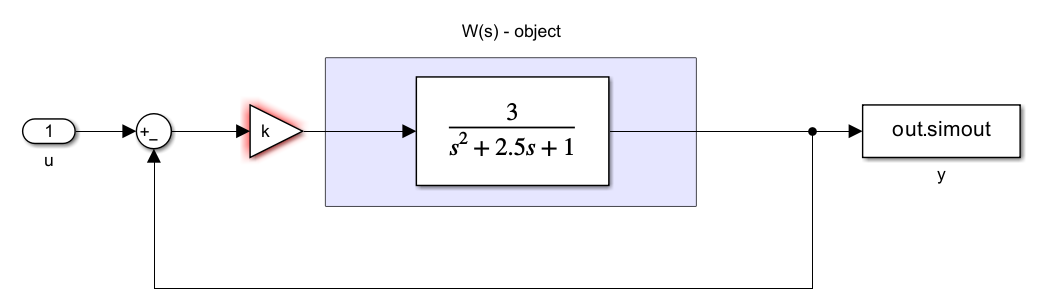
\includegraphics[width=1.0\textwidth]{scheme_system3.png}
\caption{Структурная схема - П-регулятор}
\end{figure}

\section{Стационарный режим работы}
Будем пытаться угнаться за сигналом $g(t) = A = 2$ в случае моего варианта.
Выберем следующие $k$:
$$
k_1 = 1, k_2 = 4,  k_3 = 10
$$
Аналитически определим $e_{final}$ пользуясь теоремой о предельном значении для каждого $k$:
$$
\lim_{t\to\infty} y(t) = \lim_{s\to 0}sE(s)
$$
Для начала найдём образ ошибки слежения: $E(s) = W_{g\to e}(s)G(s)$
$$
W_{g\to e} = \frac{1}{1+W(s)} = \frac{s^2 +2.5s + 1}{s^2 + 2.5s + 3k + 1}
$$
$$
G(s) = \frac{A}{s}
$$
$$
E(s) = \frac{A(s^2 +2.5s + 1)}{s(s^2 + 2.5s + 3k + 1)}
$$
В итоге:
$$
\begin{aligned}
  \lim_{t\to\infty} y(t) = \lim_{s\to 0}s\frac{A(s^2 +2.5s + 1)}{s(s^2 + 2.5s + 3k + 1)} \\
  \lim_{t\to\infty} y(t) = \lim_{s\to 0}\frac{A(s^2 +2.5s + 1)}{s^2 + 2.5s + 3k + 1} = \frac{A}{3k + 1}
\end{aligned}
$$
$$
\begin{aligned}
  e_{1} = 0.5 \\
  e_{2} = 2/13 \\
  e_{3} = 2/31 \\
\end{aligned}
$$

\begin{figure}[ht]
  \centering
  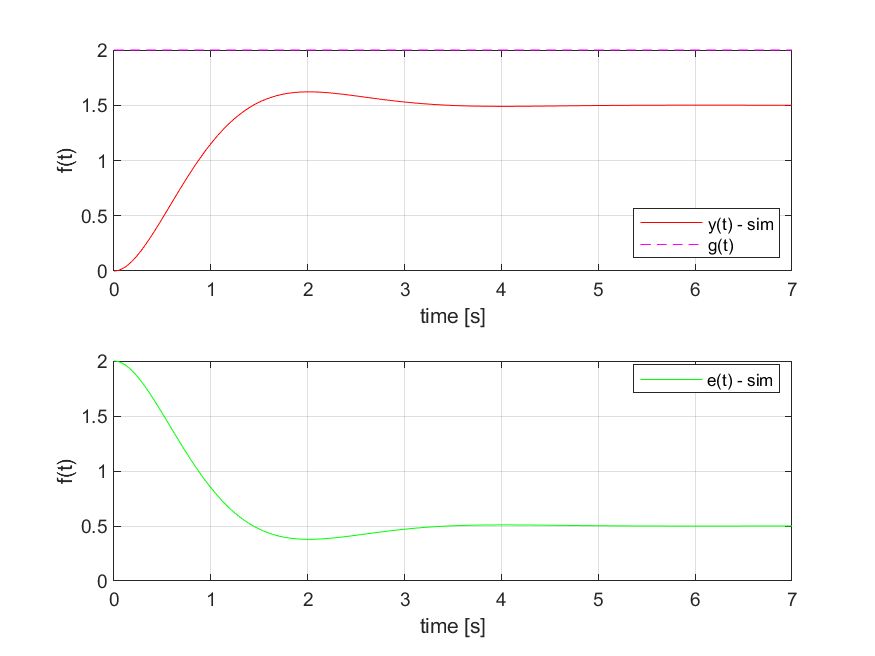
\includegraphics[width=0.8\textwidth]{output_task3_exp1.png}
\caption{Симуляция - стационарный, $k=1$}
\end{figure}

\newpage
\begin{figure}[ht]
  \centering
  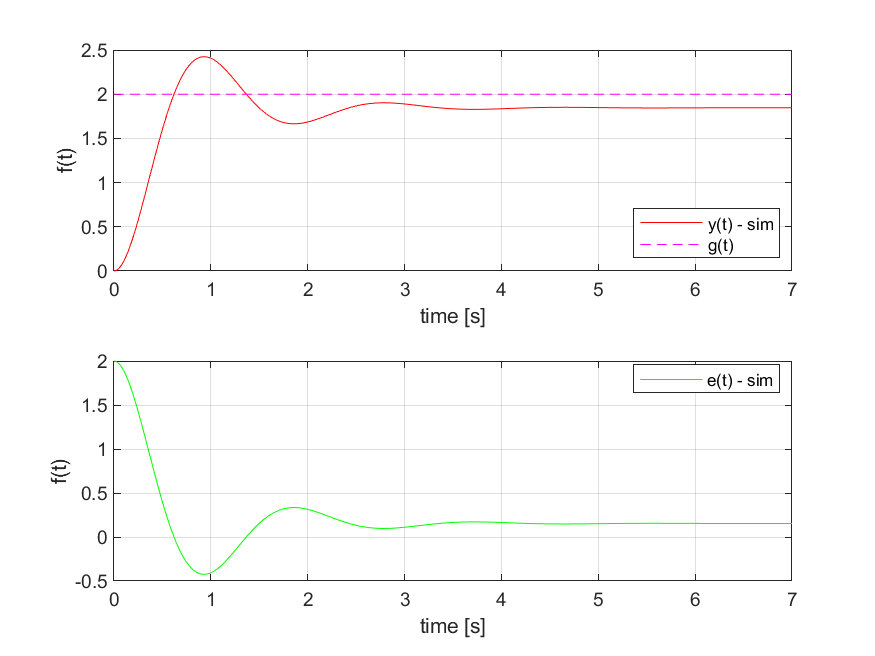
\includegraphics[width=0.8\textwidth]{output_task3_exp2.png}
\caption{Симуляция - стационарный, $k=4$}
\end{figure}

\begin{figure}[ht]
  \centering
  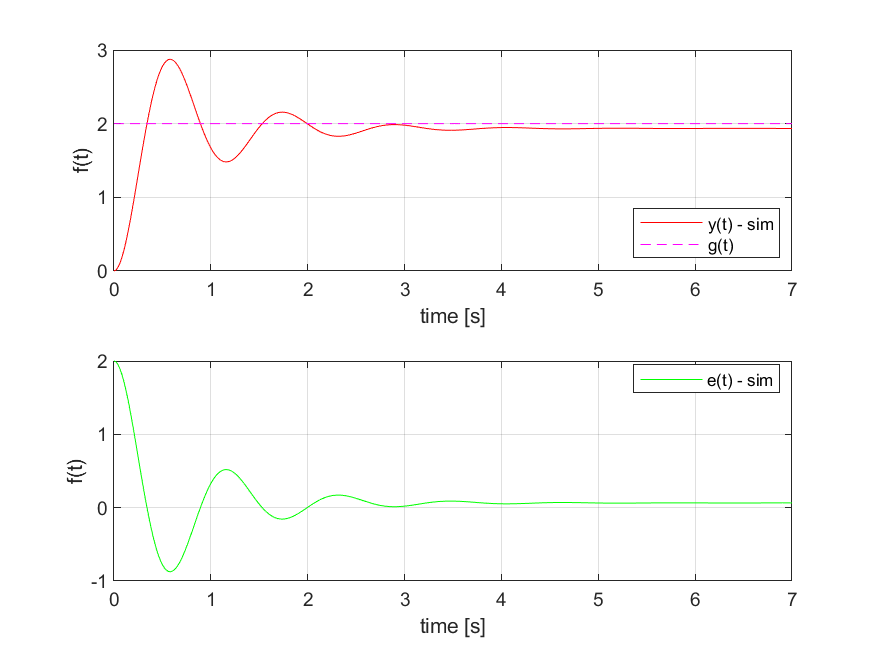
\includegraphics[width=0.8\textwidth]{output_task3_exp3.png}
\caption{Симуляция - стационарный, $k=10$}
\end{figure}

\newpage
\begin{figure}[ht]
  \centering
  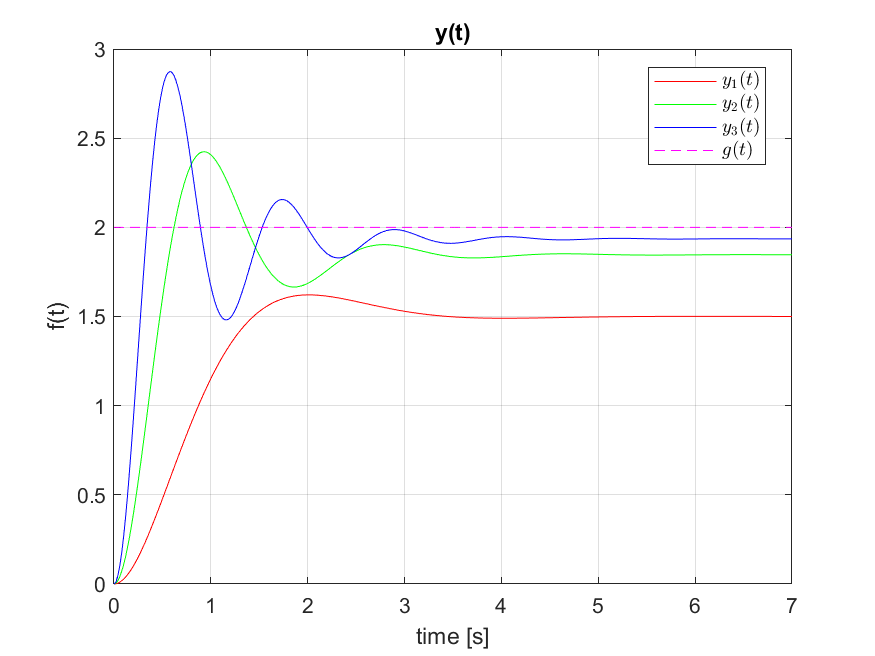
\includegraphics[width=0.8\textwidth]{output_task3_exp4.png}
\caption{Симуляция - стационарный, сравнение сигналов}
\end{figure}

\begin{figure}[ht]
  \centering
  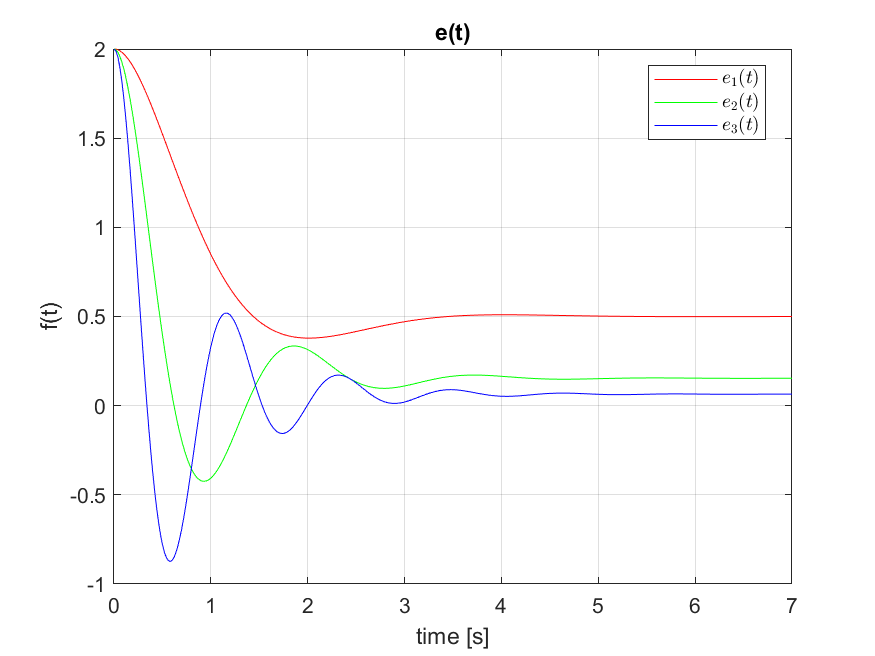
\includegraphics[width=0.8\textwidth]{output_task3_exp5.png}
\caption{Симуляция - стационарный, сравнение ошибок}
\end{figure}

\newpage
\textbf{Выводы:} при увеличении $k$ наш сигнал $y(t)$ всё больше и больше приближается к $g(t)$ с установившейся ошибкой $e_{final} = \frac{k}{3k+1}$.
Также увеличение $k$ усиливает перерегулирование при достижении цели.

\section{Движение с постоянной скоростью}
Будем пытаться угнаться за сигналом $g(t) = Vt = 2t$ в случае моего варианта.
Выберем следующие $k$:
$$
k_1 = 1, k_2 = 4,  k_3 = 10
$$

Аналитически определим $e_{final}$ пользуясь теоремой о предельном значении для каждого $k$:
$$
W_{g\to e} = \frac{1}{1+W(s)} = \frac{s^2 +2.5s + 1}{s^2 + 2.5s + 3k + 1}
$$
$$
G(s) = \frac{V}{s^2}
$$
Образ ошибки слежения:
$$
E(s) = \frac{V(s^2 +2.5s + 1)}{s^2(s^2 + 2.5s + 3k + 1)}
$$
В итоге:
$$
\begin{aligned}
  \lim_{t\to\infty} y(t) = \lim_{s\to 0}s\frac{V(s^2 +2.5s + 1)}{s^2(s^2 + 2.5s + 3k + 1)} = \infty \\
\end{aligned}
$$
А значит при любом $k$ ошибка будет улетать в бесконечность.. сигналы $y(t)$ и $g(t)$ будут расходиться

\begin{figure}[ht]
  \centering
  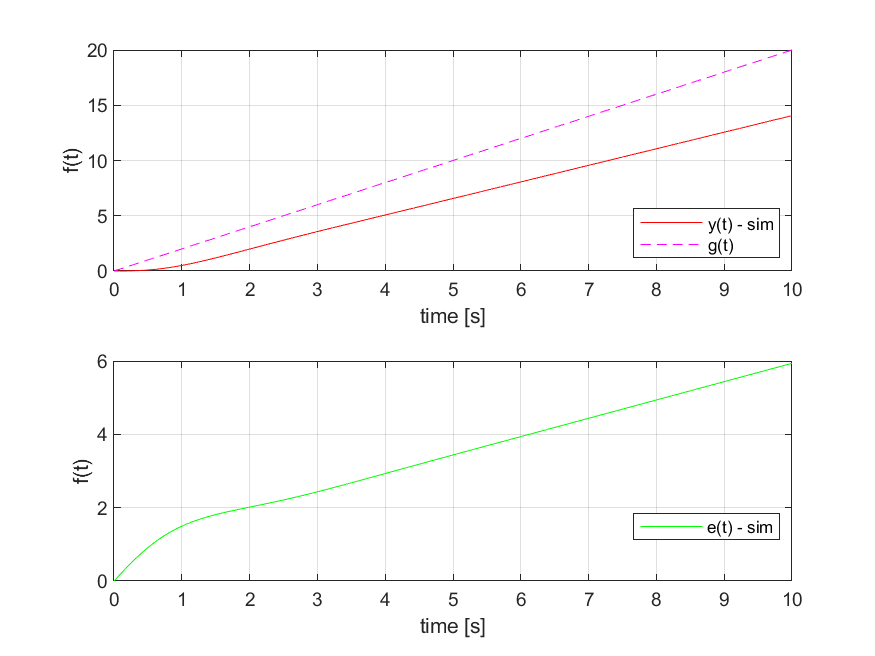
\includegraphics[width=0.8\textwidth]{output_task3_exp6.png}
\caption{Симуляция - постоянная скорость, $k=1$}
\end{figure}

\newpage
\begin{figure}[ht]
  \centering
  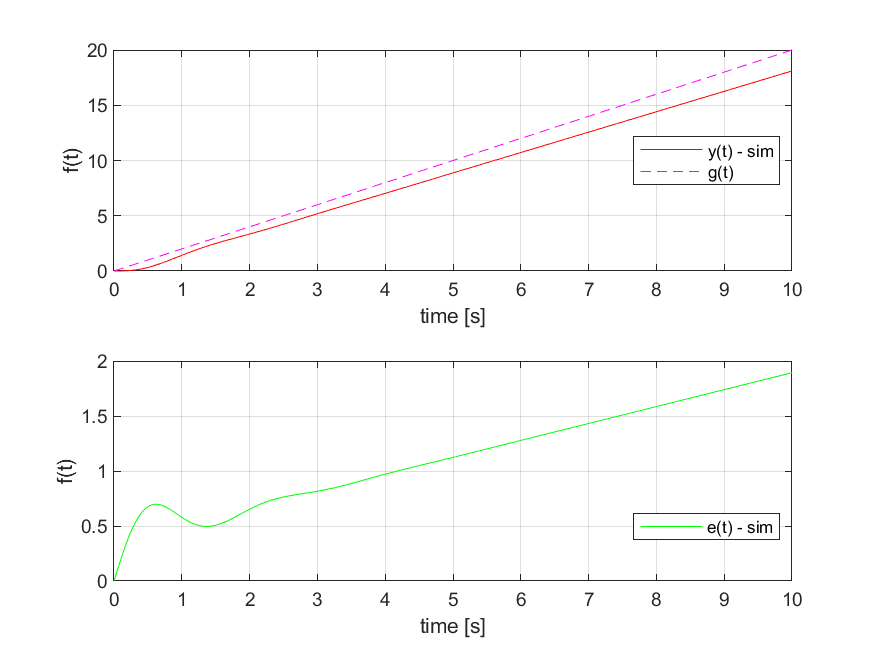
\includegraphics[width=0.8\textwidth]{output_task3_exp7.png}
\caption{Симуляция - постоянная скорость, $k=4$}
\end{figure}

\begin{figure}[ht]
  \centering
  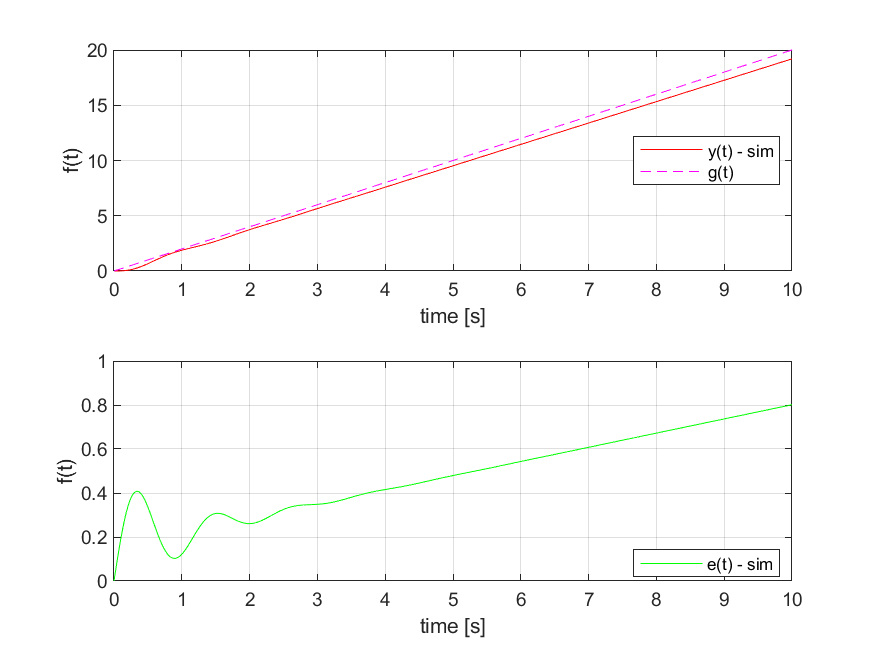
\includegraphics[width=0.8\textwidth]{output_task3_exp8.png}
\caption{Симуляция - постоянная скорость, $k=10$}
\end{figure}

\newpage
\begin{figure}[ht]
  \centering
  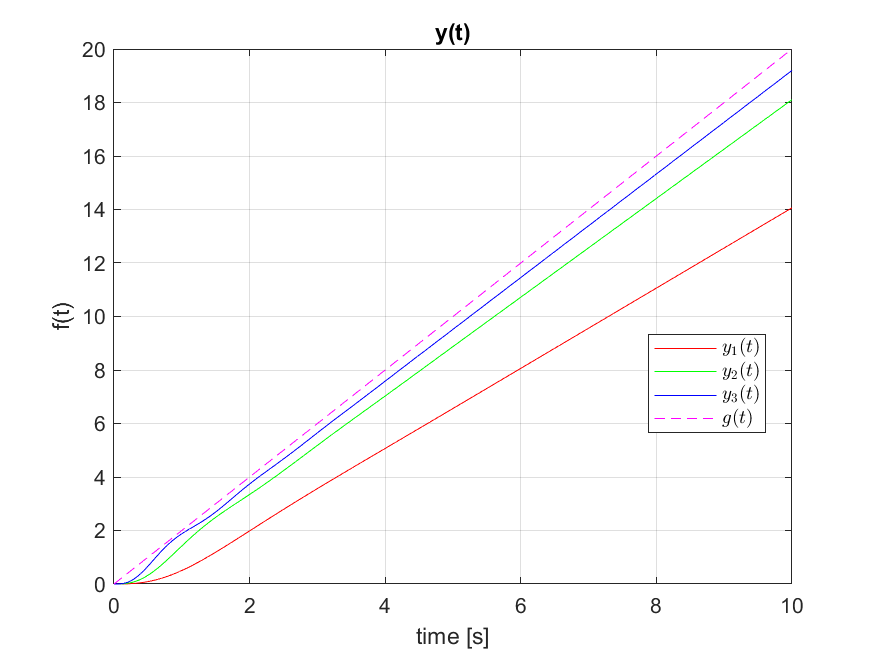
\includegraphics[width=0.8\textwidth]{output_task3_exp9.png}
\caption{Симуляция - постоянная скорость, сравнение сигналов}
\end{figure}

\begin{figure}[ht]
  \centering
  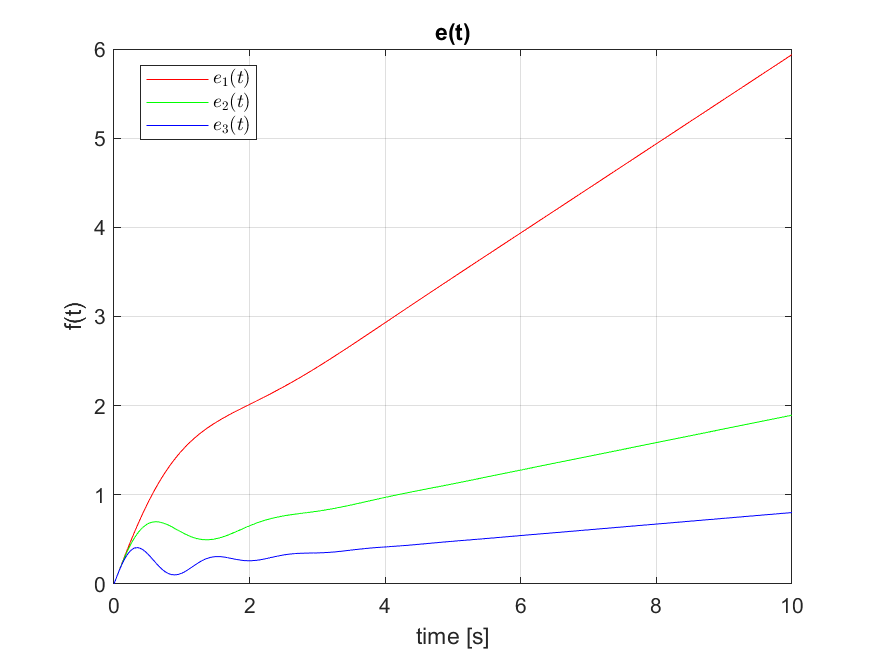
\includegraphics[width=0.8\textwidth]{output_task3_exp10.png}
\caption{Симуляция - постоянная скорость, сравнение ошибок}
\end{figure}

\newpage
\textbf{Выводы:} хоть и сигналы будут всегда расходиться, но можно заметить, что при увеличении $k$ наш сигнал $y(t)$ будет сначало достаточно близок к $g(t)$, а только потом начнёт удаляться.
Также увеличение $k$ усиливает перерегулирование при достижении цели.

\endinput